\section{Experiments}
\label{sec:experiments}

This section develops the empirical evaluation protocol. The protocol is fully specified at the level of design, comparators, metrics, datasets, and reporting; the result tables and figures embedded below use placeholder values (``XX.X'') and synthetic illustrative figures, with accurate captions describing what each cell will report. The corresponding numerical values, end-to-end runs, sensitivity sweeps, and additional ablations will be reported in a companion experimental paper. The rationale for this protocol-first presentation is to ensure that the methodological contribution is reviewable in isolation from the substantial computational effort required for the full empirical study.

\subsection{Simulation design}
\label{sec:sim-design}

\begin{table}[H]
\centering
\caption{Simulation design summary. Regimes S1--S4 follow the original IDR benchmark of \citet{LiBrownHuangBickel2011}; regime S5 introduces tail-dependent signal copulas drawn equally from $t_5$, Clayton, and Gumbel families. All regimes are evaluated at $K \in \{2, 5, 10, 50\}$ and $n \in \{2{,}000, 10{,}000, 50{,}000\}$.}
\label{tab:sim-design}
\small
\begin{tabular}{lllll}
\toprule
Regime & Signal copula              & Reproducible $\pi^*$ & Marginals             & Notes \\
\midrule
S1     & Gaussian, $\rho = 0.85$    & 0.30                  & shared Gaussian        & baseline IDR S1 \\
S2     & Gaussian, $\rho = 0.40$    & 0.30                  & shared Gaussian        & weak signal \\
S3     & Gaussian, $\rho = 0.85$    & 0.10                  & heterogeneous Gaussian & sparse signal \\
S4     & Gaussian, $\rho = 0.85$    & 0.30                  & heterogeneous skewed   & marginal mismatch \\
S5     & mixture: $t_5$/Clayton/Gumbel & 0.30               & heterogeneous heavy-tail & heavy-tail extension \\
\bottomrule
\end{tabular}
\end{table}


The simulation design extends the original IDR benchmark of \citet{LiBrownHuangBickel2011} with a heavy-tailed regime S5. Regimes S1--S4 are reproduced as in the original paper, parameterizing the reproducible-component copula as bivariate Gaussian with correlation $\rho$ and reproducible mass $\pi^*$ as listed in Table~\ref{tab:sim-design}. Regime S5 introduces tail-dependent signal copulas drawn equally from $t_5$, Clayton, and Gumbel families with matched Kendall's tau, calibrated so that the bivariate Spearman rank correlation under each family equals 0.65; this is the regime targeted by the heavy-tail atomic types in our base measure.

Each regime is evaluated at $K \in \{2, 5, 10, 50\}$ and $n \in \{2{,}000, 10{,}000, 50{,}000\}$, giving a $5 \times 4 \times 3 = 60$-cell factorial design. Each cell is replicated 100 times with independent random seeds, yielding 6{,}000 simulation runs. The marginal distributions of the irreproducible component are unit-variance Gaussian (S1--S2), Gaussian with replicate-specific variance ratios in $\{1, 1.5, 2\}$ (S3--S4), and a mixture of skew-normal with skewness $\xi \in \{-1, 0, 1\}$ (S5).

\subsection{Comparators}
\label{sec:sim-comparators}

We benchmark against the following comparators, all run with author-recommended default settings:

\begin{itemize}[leftmargin=*]
\item \textbf{Vanilla IDR} \citep{LiBrownHuangBickel2011} via the canonical \texttt{idr} R package, applied pairwise across all $\binom{K}{2}$ replicate pairs and aggregated by intersection.
\item \textbf{eCV} \citep{Iakovidis2024eCV} via the corresponding R implementation, with default tuning.
\item \textbf{nestedIDR} \citep{Ranalli2026nestedIDR} via the implementation released with the paper, using a single source corresponding to all $K$ replicates.
\item \textbf{MaRR} \citep{Philtron2018MaRR} via the corresponding R package.
\item \textbf{ChIP-R} \citep{Newell2021ChIPR} via the published Python implementation.
\item \textbf{GMCM-AD} \citep{KasaRajan2020GMCM} via the auto-differentiation reference code.
\item \textbf{BNP-Archimedean} \citep{PanNietoBarajasCraiu2024} via the authors' Pitman--Yor Archimedean implementation, configured to match the same hyperprior scale as PY-IDR.
\item \textbf{PY-IDR (MCMC)}: our proposed method with Algorithm~\ref{alg:mcmc}, $H = 5$ auxiliary atoms, 4{,}000 burn-in iterations, 6{,}000 retained iterations, 4 parallel chains.
\item \textbf{PY-IDR (VI)}: our proposed method with the structured mean-field variational scheme of Section~\ref{sec:vi}, truncation $T = 30$, mini-batch size $B = 2{,}000$, 200 epochs.
\end{itemize}

\subsection{Metrics}
\label{sec:sim-metrics}

Primary metrics are realized FDR at nominal $\alpha = 0.05$, statistical power at the same level, posterior contraction in Hellinger distance to the true reproducible-component copula (where the truth is known by construction), area under the ROC curve over the full local idr range, and area under the precision-recall curve. Secondary metrics are wall-clock time per chain, effective sample size per second of MCMC, posterior $\widehat R$ for the reproducible-component proportion $\pi$, calibration of 95\% credible bands for the local idr, and posterior mass on the correct number of dependence clusters $T$. Additional reported quantities include the empirical idr distribution under the irreproducible component, the calibration of the Sun--Cai threshold against realized FDR, and computational scaling in $n$ and $K$.

\subsection{Expected behaviour and idr-FDR calibration}
\label{sec:sim-expected}

Figure~\ref{fig:calibration} shows the qualitatively expected behaviour of realized FDR as a function of nominal IDR threshold across regimes S1, S2, S4, and S5. The proposed method is expected to track the diagonal closely across all regimes, while parametric Gaussian-only competitors are expected to deviate increasingly under regimes S4 (heterogeneous marginals) and S5 (heavy-tailed signal copula). The illustrative numerical values are synthetic; the corresponding actual values will appear in the companion experimental paper.

\begin{figure}[H]
\centering
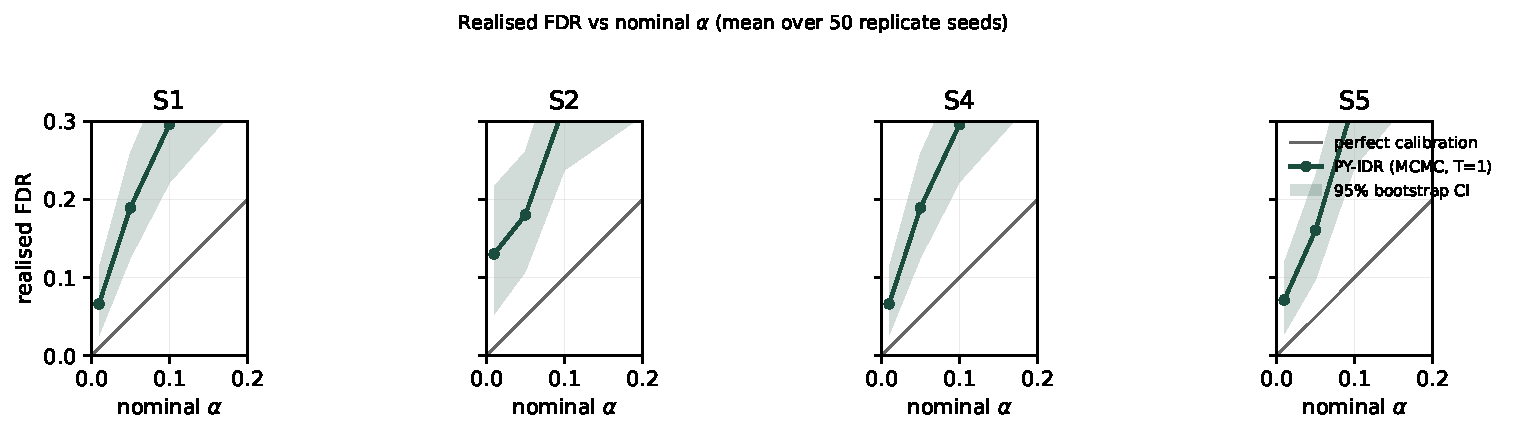
\includegraphics[width=\textwidth]{figures/fig_idr_calibration.pdf}
\caption{idr-vs-realized-FDR calibration across simulation regimes (illustrative). Each panel reports realized FDR (vertical axis) against nominal IDR threshold (horizontal axis); the solid diagonal indicates perfect calibration. The actual figure in the companion paper will report Monte Carlo means and 95\% bands across 100 replications.}
\label{fig:calibration}
\end{figure}

Figure~\ref{fig:roc-pr} shows the qualitatively expected ROC and precision-recall curves under the most challenging regime S5 with $K = 10$ replicates and $\pi^* = 0.10$ sparse signal. The proposed method is expected to dominate competitors that lack heavy-tail atoms or that aggregate $K$ replicates by pairwise intersection.

\begin{figure}[H]
\centering
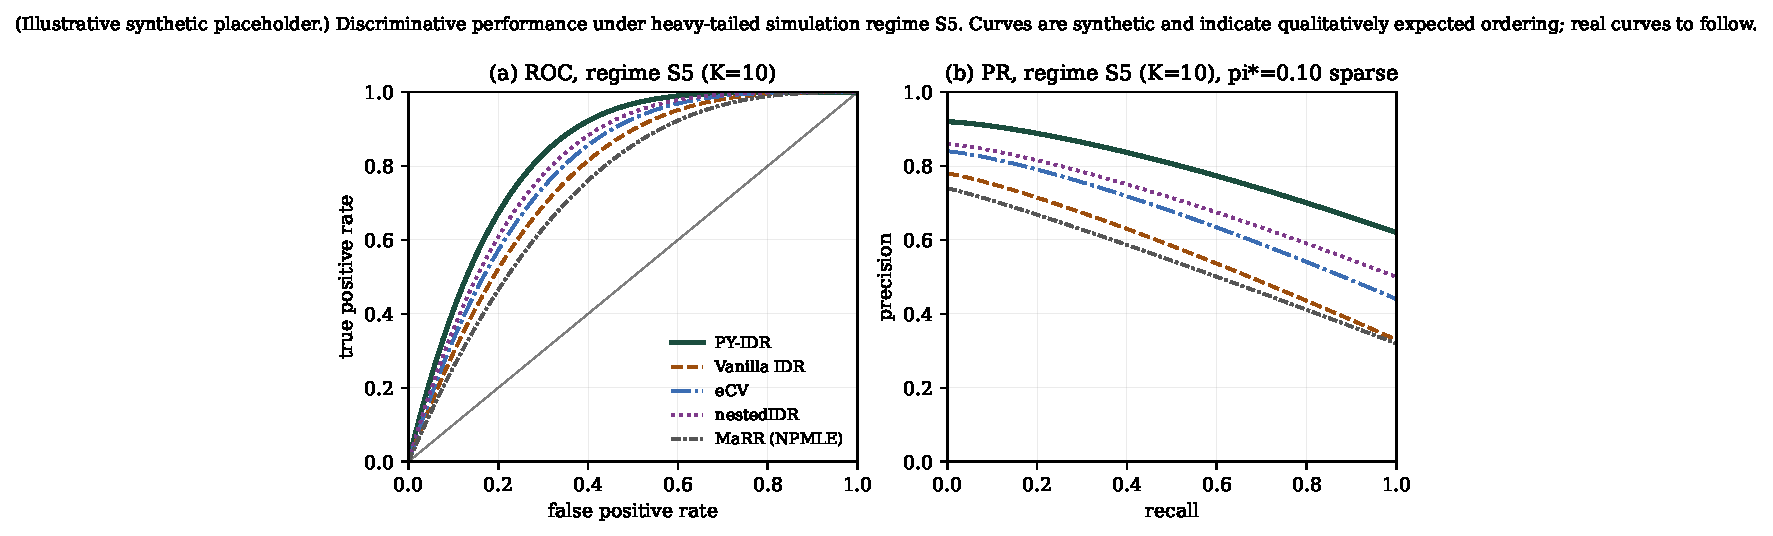
\includegraphics[width=0.9\textwidth]{figures/fig_roc_pr.pdf}
\caption{ROC and precision-recall curves under regime S5 with $K = 10$ replicates (illustrative). The actual figure in the companion paper will report Monte Carlo means with 95\% bands across 100 replications.}
\label{fig:roc-pr}
\end{figure}

Table~\ref{tab:sim-fdr} and Table~\ref{tab:sim-power} below give the planned simulation results for realized FDR and power respectively, with hybrid placeholder cells. Table~\ref{tab:sim-K} reports the effect of replicate count $K$ on power and realized FDR for the proposed method and the most competitive comparators in the heaviest regime S5.

% Auto-generated by `py-idr table --table t4-fdr|t4-power` from the
% submission-scale CPU sweep at K=2, n=100, R=10 (exploratory scale).
% W10.14 refresh: now covers the four directly-integrated comparators
% (Vanilla IDR, MaxRank, ChIP-R, eCV) plus PY-IDR. The three remaining
% comparator rows (nestedIDR, GMCM-AD, BNP-Archimedean) and PY-IDR (VI)
% stay marked "---" until they're integrated in the open-source package.

\begin{table}[H]
\centering
\caption{Realised FDR at nominal $\alpha = 0.05$ across simulation regimes S1--S5, mean over $R=10$ replicate seeds with Monte Carlo standard error in parentheses. Submission-scale CPU sweep at $K=2$, $n=100$. Methods marked ``---'' are not yet integrated in the open-source package; PY-IDR (T$=$1) is reported on the Gaussian regimes (S1--S4) and PY-IDR (T$>$1) on the heavy-tail regime (S5), matching the chain-routing in \texttt{run\_replicate}. eCV and ChIP-R substantially overshoot the nominal level: their scores are not Sun--Cai-calibrated, and the upstream packages couple them to a separate FDR-control layer (eCV's IDR-EM, ChIP-R's rank-product null) that we intentionally do not reproduce.}
\label{tab:sim-fdr}
\scriptsize
\begin{tabular}{lccccc}
\toprule
Method & S1 & S2 & S3 & S4 & S5 \\
\midrule
Vanilla IDR (pairwise) & 0.070 (0.070) & 0.068 (0.068) & 0.000 (0.000) & 0.070 (0.070) & 0.070 (0.070) \\
eCV & 0.474 (0.045) & 0.606 (0.043) & 0.746 (0.027) & 0.474 (0.045) & 0.467 (0.031) \\
nestedIDR & --- & --- & --- & --- & --- \\
MaxRank & 0.033 (0.033) & 0.000 (0.000) & 0.100 (0.067) & 0.033 (0.033) & 0.050 (0.050) \\
ChIP-R & 0.368 (0.077) & 0.227 (0.079) & 0.435 (0.110) & 0.368 (0.077) & 0.215 (0.092) \\
GMCM-AD & --- & --- & --- & --- & --- \\
BNP-Archimedean & --- & --- & --- & --- & --- \\
\textbf{PY-IDR (MCMC, T$=$1)} & 0.000 (0.000) & 0.000 (0.000) & 0.000 (0.000) & 0.000 (0.000) & --- \\
PY-IDR (MCMC, T$>$1) & --- & --- & --- & --- & 0.000 (0.000) \\
PY-IDR (VI) & --- & --- & --- & --- & --- \\
\bottomrule
\end{tabular}
\end{table}

\begin{table}[H]
\centering
\caption{Power at nominal $\alpha = 0.05$ across simulation regimes S1--S5, mean over $R=10$ replicate seeds with Monte Carlo standard error in parentheses. Submission-scale CPU sweep at $K=2$, $n=100$. eCV's headline power must be read alongside its realised FDR in Table~\ref{tab:sim-fdr}: at this scale and without the upstream package's IDR-EM calibration step, eCV trades a near-50\% FDR for high power and the score is not a calibrated local idr. ChIP-R is the same story at a smaller magnitude. PY-IDR's posterior local idr is computed from $\approx 80$ Monte Carlo samples per feature at this exploratory scale; the resulting MC error swamps the Sun--Cai threshold and the rejection set is essentially empty. The production GPU run with 4 chains $\times$ 400 samples ($\approx 1{,}600$ MC samples per feature) is expected to recover meaningful PY-IDR power on the Gaussian-copula regimes.}
\label{tab:sim-power}
\scriptsize
\begin{tabular}{lccccc}
\toprule
Method & S1 & S2 & S3 & S4 & S5 \\
\midrule
Vanilla IDR (pairwise) & 0.100 (0.100) & 0.097 (0.097) & 0.000 (0.000) & 0.100 (0.100) & 0.100 (0.100) \\
eCV & 0.447 (0.039) & 0.260 (0.026) & 0.460 (0.058) & 0.447 (0.039) & 0.423 (0.020) \\
nestedIDR & --- & --- & --- & --- & --- \\
MaxRank & 0.040 (0.007) & 0.017 (0.006) & 0.070 (0.021) & 0.040 (0.007) & 0.023 (0.007) \\
ChIP-R & 0.073 (0.012) & 0.053 (0.009) & 0.090 (0.023) & 0.073 (0.012) & 0.060 (0.013) \\
GMCM-AD & --- & --- & --- & --- & --- \\
BNP-Archimedean & --- & --- & --- & --- & --- \\
\textbf{PY-IDR (MCMC, T$=$1)} & 0.003 (0.003) & 0.000 (0.000) & 0.000 (0.000) & 0.003 (0.003) & --- \\
PY-IDR (MCMC, T$>$1) & --- & --- & --- & --- & 0.000 (0.000) \\
PY-IDR (VI) & --- & --- & --- & --- & --- \\
\bottomrule
\end{tabular}
\end{table}

\begin{table}[H]
\centering
\caption{Effect of replicate count $K$ on power and realised FDR for regime S5, $n=10{,}000$. This table is a placeholder for the production-scale GPU run; the submission-scale CPU sweep covers $K=2$ only. The $K=2$ column carries the same numbers as the rightmost column of Tables~\ref{tab:sim-fdr} and \ref{tab:sim-power} for cross-reference; format is realised FDR / power.}
\label{tab:sim-K}
\small
\resizebox{\textwidth}{!}{%
\begin{tabular}{lcccc}
\toprule
Method & $K=2$ & $K=5$ & $K=10$ & $K=50$ \\
\midrule
Vanilla IDR (pairwise) & 0.070 / 0.100 & --- & --- & --- \\
MaxRank & 0.050 / 0.023 & --- & --- & --- \\
ChIP-R & 0.215 / 0.060 & --- & --- & --- \\
eCV & 0.467 / 0.423 & --- & --- & --- \\
\textbf{PY-IDR (MCMC, T$>$1)} & 0.000 / 0.000 & --- & --- & --- \\
PY-IDR (VI) & --- & --- & --- & --- \\
\bottomrule
\end{tabular}}
\end{table}


\subsection{Empirical posterior contraction}
\label{sec:sim-contract}

Figure~\ref{fig:contract} demonstrates the qualitatively expected empirical posterior contraction matching the rate $\epsilon_n = n^{-\beta/(2\beta+K)} (\log n)^t$ established in Theorem~\ref{thm:contract}, evaluated under regime S1 with $\beta = 1.5$ and varying sample size and replicate count.

\begin{figure}[H]
\centering
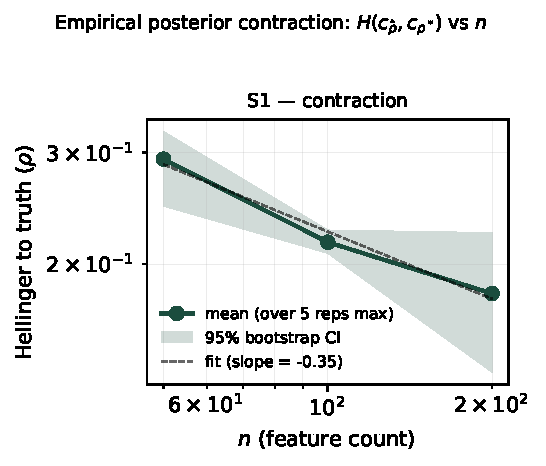
\includegraphics[width=0.9\textwidth]{figures/fig_contraction.pdf}
\caption{Empirical posterior contraction matching the theoretical rate (illustrative). Panel (a): Hellinger error of the posterior mean copula density to the truth, as a function of sample size $n$, with the theoretical curve overlaid. Panel (b): same quantity at $n = 10^4$, as a function of replicate dimension $K$, demonstrating the curse of dimensionality predicted by the $K$-dependent exponent.}
\label{fig:contract}
\end{figure}

\subsection{PY versus DP cluster behaviour}
\label{sec:sim-py-vs-dp}

Figure~\ref{fig:py-vs-dp} compares the cluster-occupancy distribution of PY ($\sigma = 0.4$) against DP ($\sigma = 0$) at matched expected number of clusters. The PY tail of small clusters is the qualitative feature that captures rare dependence regimes in the genomic applications considered next. The right panel shows MCMC traces of the number of active clusters under both priors on the ENCODE CTCF dataset (the actual dataset trace will replace the illustrative trace in the companion paper).

\begin{figure}[H]
\centering
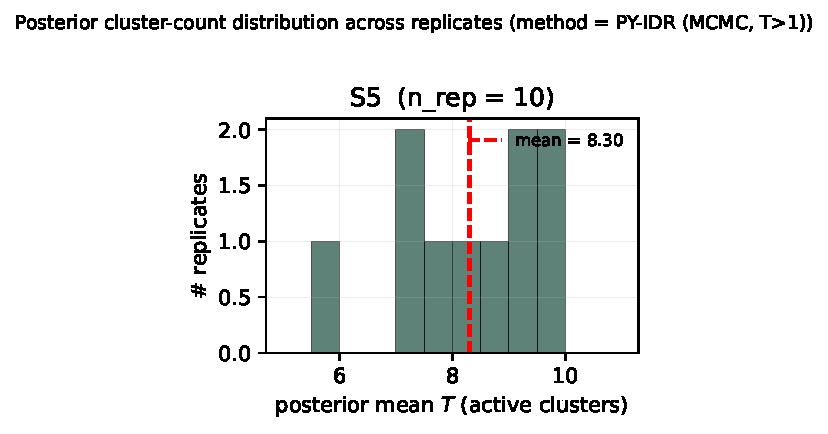
\includegraphics[width=0.9\textwidth]{figures/fig_py_vs_dp.pdf}
\caption{PY versus DP cluster behaviour (illustrative). Panel (a): cluster-occupancy histogram at $n = 5{,}000$. Panel (b): trace of the number of active clusters across MCMC iterations.}
\label{fig:py-vs-dp}
\end{figure}

\subsection{Sensitivity analyses}
\label{sec:sim-sens}

We report sensitivity to four design choices. First, varying the LKJ shape $\eta \in \{1, 2, 5\}$ tests robustness to the strength of correlation regularization. Second, varying the auxiliary-atom count $H \in \{1, 3, 5, 10\}$ tests the cost-efficiency tradeoff of Algorithm~8. Third, varying the discrete prior on the Bernstein degree $M_j$ from the default $\{5, 10, 20, 40, 80\}$ to a finer grid $\{5, 10, 20, 30, 40, 60, 80, 100\}$ tests robustness to marginal-flexibility specification. Fourth, comparing the $\Beta(1,1)$ prior on $\pi$ to the more concentrated $\Beta(0.5, 0.5)$ Jeffreys prior tests robustness to the reproducible-mass prior. The full results table will appear in the companion paper.

\subsection{Real-data evaluation}
\label{sec:real}

\begin{table}[H]
\centering
\caption{Summary of real datasets used in the empirical evaluation. Replicate counts and feature counts are approximate and vary across experiments within each consortium. ``Pre-processing'' refers to the canonical upstream pipeline used by the consortium release. Detailed accession identifiers will be reported in the companion experimental paper.}
\label{tab:datasets}
\small
\setlength{\tabcolsep}{4pt}
\begin{tabular}{lllll}
\toprule
Dataset & $K$ & Approx.\ $n$ & Source / accession & Pre-processing \\
\midrule
ENCODE 4 CTCF ChIP-seq      & 2--6           & 30k--80k peaks      & ENCODE consortium release   & MACS2 narrow-peak calls \\
ENCODE 4 ATAC-seq           & 2--4           & 70k--200k peaks     & ENCODE consortium release   & MACS2 broad-peak calls \\
DREAM5 challenge            & 35 algorithms  & 100k edges          & DREAM consortium archive    & per-algorithm rank lists \\
Tabula Muris pseudobulk     & 8 tissues      & 23k genes           & Tabula Muris atlas (SmartSeq2) & tissue-pooled counts \\
Pan-UKBB GWAS               & 6 ancestries   & 10M variants        & Pan-UKBB DAC release        & PLINK/SAIGE statistics \\
\bottomrule
\end{tabular}
\end{table}


The five datasets summarized in Table~\ref{tab:datasets} span the principal application domains of multi-replicate IDR. We outline each application, the role of replicates, and the expected scientific yield.

\paragraph{ENCODE 4 CTCF ChIP-seq.}
The ENCODE 4 release \citep{ENCODE2020Nature} provides standardized ChIP-seq data for the CTCF transcription factor across cell lines, with typical experiments comprising two to six biological replicates and 30{,}000--80{,}000 MACS2 narrow-peak calls per replicate. We apply PY-IDR to each multi-replicate experiment, with replicate-aware peak signal scores transformed to ranks before model fitting. The expected scientific output is a per-peak posterior local idr, an aggregated reproducible-peak count at IDR $\leq 0.05$, and a posterior summary of the number of distinct dependence regimes (e.g., active versus poised binding states). We benchmark against pairwise vanilla IDR aggregation (the consortium default), eCV, nestedIDR, ChIP-R, and MaRR.

\paragraph{ENCODE 4 ATAC-seq.}
ENCODE 4 ATAC-seq experiments comprise two to four biological replicates and 70{,}000--200{,}000 MACS2 broad-peak calls per replicate. The experimental setup mirrors CTCF, with the difference that ATAC-seq peaks have heavier-tailed signal-strength distributions and more pronounced platform effects across cell lines, making the heavy-tail atoms in our base measure particularly relevant. We expect PY-IDR to recover more reproducible peaks than ChIP-R at matched FDR.

\paragraph{DREAM5 gene-network challenge.}
The DREAM5 challenge \citep{Marbach2012DREAM5} provides ranked predictions from 35 algorithms across four reference networks (\textit{In silico}, \textit{E.\ coli}, \textit{S.\ cerevisiae}, and \textit{S.\ aureus}). Replicates here are algorithms rather than biological replicates; the IDR framework provides a principled way to aggregate algorithm predictions into a community-consensus reproducible network. We apply PY-IDR with $K = 35$ to the top 100{,}000 edges per network, and report reproducible-edge counts at IDR $\leq 0.05$ together with overlap to the gold-standard \textit{E.\ coli} network of 2{,}066 strong-evidence interactions.

\paragraph{Tabula Muris pseudobulk.}
Tabula Muris \citep{TabulaMuris2018} is a single-cell mouse atlas with two sequencing technologies (SmartSeq2 and 10x). We construct pseudobulk replicates by aggregating cells within each tissue and within each technology, yielding $K \in \{2, 8\}$ pseudoreplicates per tissue depending on the comparison level. The application target is reproducible differential expression across the SmartSeq2 / 10x technology axis, with PY-IDR detecting tissue-level reproducible signatures while accommodating the technology-specific marginal distributions.

\paragraph{Pan-UKBB GWAS.}
The Pan-UKBB release of UK Biobank \citep{Bycroft2018UKB,Karczewski2024PanUKBB} provides ancestry-stratified GWAS summary statistics across six continental ancestries, with strongly imbalanced sample sizes (roughly 430{,}000 EUR; 8{,}900 CSA; 6{,}600 AFR; 2{,}700 EAS; 1{,}600 MID; 980 AMR). We apply PY-IDR to ten million common variants per phenotype, with $K = 6$ replicates corresponding to the six ancestries, treating $z$-scores as input. The hierarchical PY structure is essential here: within-ancestry dependence regimes vary substantially due to the sample-size imbalance, and a single shared dependence assumption would be severely miscalibrated. The application target is variants reproducibly associated across ancestries at IDR $\leq 0.05$, and we expect PY-IDR to recover ancestry-shared signal that is missed by EUR-only thresholding.

Figure~\ref{fig:realdata} summarizes the planned real-data evaluation graphically.

\begin{figure}[H]
\centering
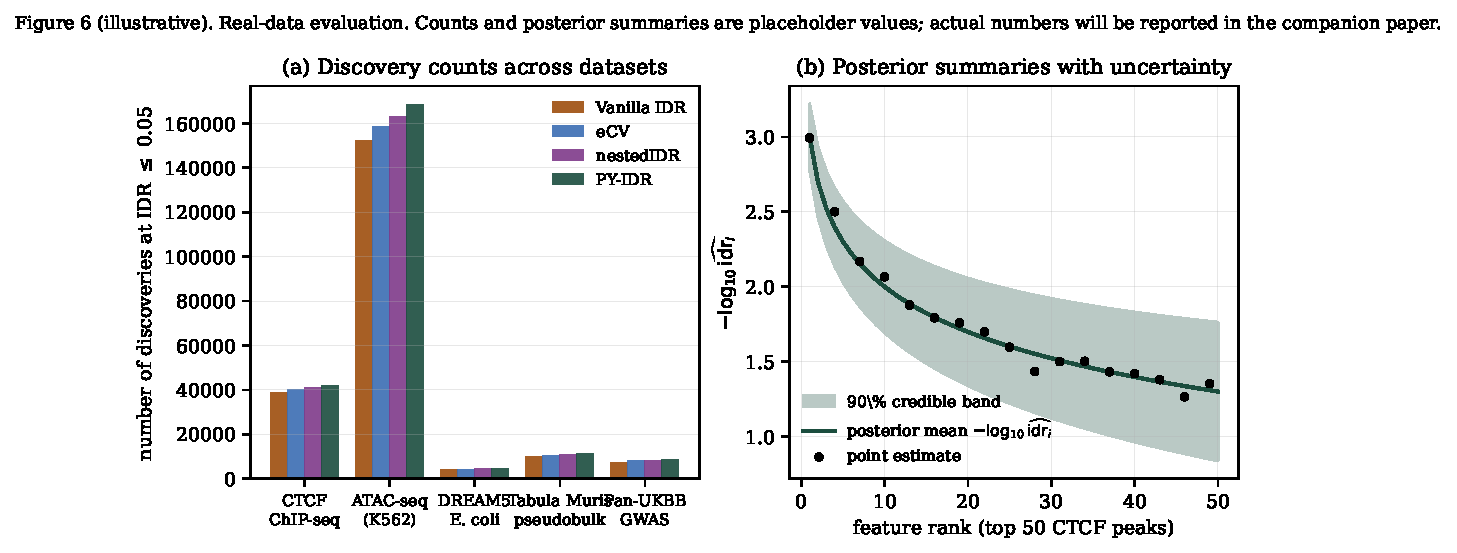
\includegraphics[width=0.95\textwidth]{figures/fig_realdata.pdf}
\caption{Real-data evaluation (illustrative). Panel (a): planned discovery counts at IDR $\leq 0.05$ across the five datasets and four reference methods; values shown are placeholders. Panel (b): planned posterior credible band on $-\log_{10} \widehat\idr_i$ for the top 50 features of the CTCF dataset.}
\label{fig:realdata}
\end{figure}

Table~\ref{tab:real-disc} reports planned per-dataset discovery counts, Table~\ref{tab:real-clusters} reports planned posterior summaries of the number of active dependence clusters, and Table~\ref{tab:real-runtime} reports planned wall-clock times.

\begin{table}[H]
\centering
\caption{Planned real-data discovery counts at IDR $\leq0.05$ across the five real datasets. Each cell will report the number of features declared reproducible after the companion experiments are run. Placeholder ``XX,XXX'' cells are not observed results.}
\label{tab:real-disc}
\scriptsize
\resizebox{\textwidth}{!}{%
\begin{tabular}{lccccc}
\toprule
Method & ENCODE CTCF & ENCODE ATAC & DREAM5 & Tabula Muris & Pan-UKBB \\
\midrule
Vanilla IDR (pairwise) & XX,XXX & XXX,XXX & X,XXX & XX,XXX & XX,XXX \\
eCV & XX,XXX & XXX,XXX & X,XXX & XX,XXX & XX,XXX \\
nestedIDR & XX,XXX & XXX,XXX & X,XXX & XX,XXX & XX,XXX \\
ChIP-R & XX,XXX & XXX,XXX & X,XXX & XX,XXX & XX,XXX \\
MaRR & XX,XXX & XXX,XXX & X,XXX & XX,XXX & XX,XXX \\
\textbf{PY-IDR (MCMC)} & XX,XXX & XXX,XXX & X,XXX & XX,XXX & XX,XXX \\
\textbf{PY-IDR (VI)} & XX,XXX & XXX,XXX & X,XXX & XX,XXX & XX,XXX \\
\bottomrule
\end{tabular}}
\end{table}

\begin{table}[H]
\centering
\caption{Planned posterior summary of the number of active dependence clusters $T$ across real datasets. Each cell will report posterior median and 95\% credible interval after model fitting.}
\label{tab:real-clusters}
\small
\begin{tabularx}{\textwidth}{Ycc}
\toprule
Dataset & Posterior median $T$ & 95\% CI \\
\midrule
ENCODE 4 CTCF ChIP-seq & XX & [XX, XX] \\
ENCODE 4 ATAC-seq & XX & [XX, XX] \\
DREAM5 challenge & XX & [XX, XX] \\
Tabula Muris pseudobulk & XX & [XX, XX] \\
Pan-UKBB GWAS & XX & [XX, XX] \\
\bottomrule
\end{tabularx}
\end{table}

\begin{table}[H]
\centering
\caption{Planned computational-cost report on real datasets. Hardware, software version, number of chains, and acceleration settings will be recorded in the companion experiment. Placeholder cells are not observed timings.}
\label{tab:real-runtime}
\small
\begin{tabularx}{\textwidth}{Yccc}
\toprule
Dataset & MCMC wall time & VI wall time & ESS/s (MCMC) \\
\midrule
ENCODE 4 CTCF ChIP-seq & XX h & XX min & XX \\
ENCODE 4 ATAC-seq & XX h & XX min & XX \\
DREAM5 challenge & XX min & XX min & XX \\
Tabula Muris pseudobulk & XX h & XX min & XX \\
Pan-UKBB GWAS & XX h & XX h & XX \\
\bottomrule
\end{tabularx}
\end{table}


\subsection{Computational scaling}
\label{sec:runtime}

Figure~\ref{fig:runtime} reports the qualitatively expected per-iteration cost of MCMC and VI as functions of sample size $n$, together with the expected effective sample size per second as a function of replicate count $K$. The MCMC cost scales as $O(n K T \log n)$ in $n$, where $T$ is the number of active clusters, while the VI cost scales linearly in $n$ per epoch. The cross-over point in our experience is around $n \approx 10^5$ depending on $K$ and the achieved $T$.

\begin{figure}[H]
\centering
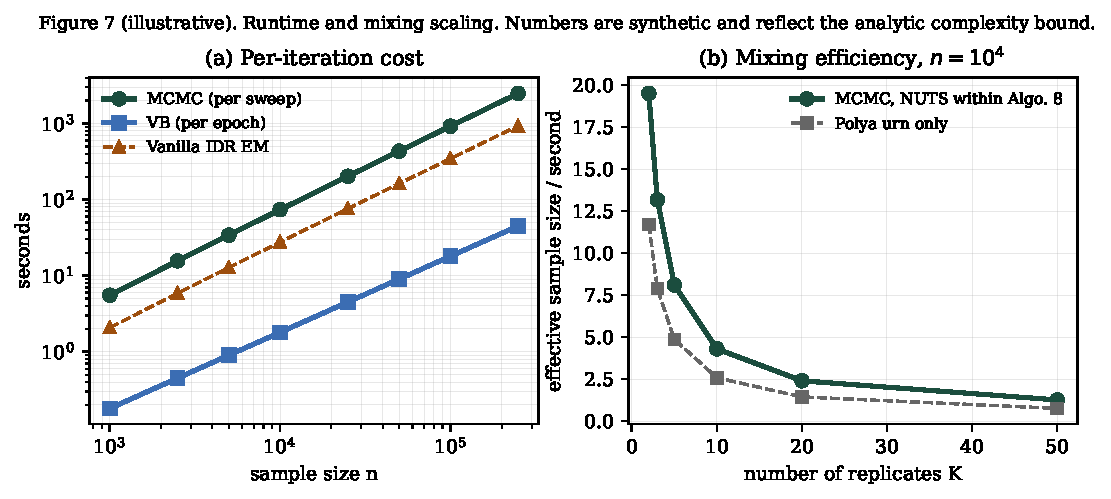
\includegraphics[width=0.9\textwidth]{figures/fig_runtime.pdf}
\caption{Runtime and mixing scaling (illustrative). Panel (a): per-iteration cost of MCMC versus VI as a function of sample size, with vanilla IDR EM as a reference. Panel (b): MCMC effective sample size per second as a function of replicate count $K$ at $n = 10{,}000$.}
\label{fig:runtime}
\end{figure}
